%\iffalse
\documentclass[%
 aip,
% jmp,
% bmf,
% sd,
% rsi,
cp,  % Conference Proceedings
 amsmath,amssymb,%nobibnotes,
% preprint,%
 reprint,%
%author-year,%
%author-numerical,%
]{revtex4-2}
%\fi

\iffalse
\documentclass{article} 
\usepackage{amsfonts,amsmath}
\usepackage{aip}
\usepackage{cp}
\usepackage{reprint}
\fi

\usepackage{graphicx}% Include figure files
\usepackage{dcolumn}% Align table columns on decimal point
\usepackage{bm}% bold math
%\usepackage[mathlines]{lineno}% Enable numbering of text and display math
%\linenumbers\relax % Commence numbering lines

\usepackage[utf8]{inputenc}
\usepackage[T1]{fontenc}
%% Loads a Times-like font. You can also load
%% {newtxtext,newtxtmath}, but not {times}, 
%% {txfonts} nor {mathtpm} as these packages
%% are obsolete and have been known to cause problems.
\usepackage{mathptmx} 
\usepackage{multirow}
\usepackage{float}

\newcommand{\be}{\begin{equation}}
\newcommand{\ee}{\end{equation}}
\newcommand{\rf}[1]{(\ref{#1})}
\newcommand{\RR}{\mathbb{R}}
\newtheorem{thm}{Theorem}
\newtheorem{lm}{Lemma}

\begin{document}

\title{Numerical Study of the good 1D Boussinesq Equation}% Force line breaks with \\

\author{...} % Write as First name Surname
 \email[Corresponding author: ]{angelow@math.bas.bg}
\affiliation{
Institute of Mathematics and Informatics\\
Bulgarian Academy of Sciences, Acad.\\
G.~Bonchev Bl.8, 1113, Sofia,
Bulgaria
}

\date{\today} % It is always \today, today, but any date may be explicitly specified
              % Not printed for conference proceedings

\begin{abstract}
In this paper we evaluate propagating wave solutions to the one-dimensional good Boussinesq Equation (BE).
Two numerical methods are used to obtain a solution. The first is a conservative finite difference scheme, and the second exploits Taylor series expansions around the time variable $t$. 
The solutions are computed over nested meshes to examine the convergence of both approaches. The main tool for testing the convergence rate of all examined finite difference schemes and Taylor expansions is the Runge's method.  It is shown that for a fixed time interval the numerical methods preserve the shape, mass and maximum of the solution. The waves obtained by the two methods are compared.
Both methods produce similar results in case of $O(h^{2} + \tau^2 )$ approximation order. The outcome of the comparison is very good. The maximum difference between the two approaches (among calculated solutions using different parameter sets) in $L_2$ and infinity norms is $???$ and $???$ respectively.

\end{abstract}

\maketitle

\section{\label{sec:level1}Introduction}

The Boussinesq type equations are famous with the approximation of shallow water waves or also weakly non--linear long waves. It is often used for simulation of various physical processes e.g. turbulence in fluid mechanics, vibrations in acoustics, etc. For the numerical interaction of 2D Boussinesq traveling waves (TW) one needs the shape of a stationary wave in order to build the Initial Condition (IC) $u_0$, $u_1$.

The shallow water model developed by Boussinesq and the equaitons he derived in this conjuction were first described in \cite{ref0}. The equation is known to have an explicit solution in the case of one moving solitary wave. It is also known that it has a solution with two solitary waves that results in their temporary combination and subsequent reemergence in their original forms after the interaction. An improvement of the Boussinesq model was done by Christov's "energy-consistent approximation" \cite{ref1} a.k.a the Boussinesq Paradigm Equation (BPE). Christov states that the original model with the initial value problem defined by Boussinesq is incorect in the sense of Hadamard (see \cite{ref1}), i.e. even small perturbations in the initial or boundary conditions could lead to significant differences in the behavior of the solution over time. Unfortunately the BPE is not known to posses an explicit solution in the case of two solitary waves. We would like to compare the numerical and the exact solutions in the case of two solitary waves. This could be done in the case of the original (a.k.a good) Boussinesq model:


\begin{align}\label{orgBsq}
&\frac{\partial^2 }{\partial t^2}u(x,t)= \frac{\partial^2}{\partial x^2}u(x,t) -  \beta_2 \frac{\partial^4}{\partial x^4}u(x,t) - \alpha\frac{\partial^2}{\partial x^2} (u(x,t)^2)
\\
&u(x,0) = u_0(x), \quad \frac{\partial }{\partial t}u(x,0)=u_1(x), \nonumber
\\
&u(x,t) \rightarrow 0, \quad \frac{\partial }{\partial t} u(x, t) \rightarrow 0 \quad \text{for} \quad |x| \rightarrow \infty \nonumber
\end{align}
where $\alpha>0$ is the amplitude and $\beta_2$  is the dispersion parameter. The domain of the unknown function $u$ is defined by:
\be
 u:\Omega \times [0, T] \rightarrow \RR,
\ee
where $\Omega \equiv (-\infty, \infty)$ and $T>0$. The continuous energy of the solution is defined by

\begin{eqnarray}\label{con-cont2}
E\left( u(x,t)\right)=	\frac{1}{2} \left\|(-\partial^2_x)^{-1/2} \frac{\partial u}{\partial t}(x,t)\right\|^2 + \frac{1}{2}  \left\|u (x,t)\right\|^2 
+ \beta_2 \frac{1}{2}\left\| \nabla u(x,t) \right\|^2+\alpha \int _{R} \int_0 ^{u(x,t)} f(s) ds dx,
\end{eqnarray}

where $f(s) = s^2$. Equation \rf{orgBsq} is equivalent to the BPE if the mixed time and space derivative is omited. E.g. if we set $\beta_1 = 0$ in equation (2) from article \cite{ref21} (Chertock, Christov, Kurganov) then it is equivalent to \rf{orgBsq} defined above. The other parameters $\beta_2 = 1$ and $\alpha = 3$ are chosen in such way so that \rf{orgBsq} obtains two wave soliton solution (see formula \rf{orgBsqSol} defined in section Numerical Results).
The soliton is localized wave, which moves at constant velocity ($\omega_i, \: i=1,2$ in case of \rf{orgBsqSol}) and maintains its shape. When a soliton interacts with another soliton, it emerges from the "collision" unchanged, i.e. its amplitude, shape, and velocity are conserved. The results and observations in the conducted numerical analysis for the good Boussinesq equation \rf{orgBsq} could be further used in order to find a two wave solitary solution for the 1D and 2D BPE.

The paper is organized as follows. Section 2 introduces the numerical methods that are used for equation \rf{orgBsq}: Method with Conservative FDS and Taylor Method which uses TS expansions around the time variable $t$. Furthermore, for each method the mass of the solution is calculated. The solution and its properties from the two methods are compared. The numerical calculations are done over nested meshes to examine the convergence of both methods. The goal is to justify the TS approach by showing that both methods exhibit similar results. Furthermore the TS method could be used with higher approximation order which produces finer solution.Section 3 concerns the numerical results. Section 3.1 shows the convergence speed of the implemented algorithms measured with Runge's rule. Section 3.2 compares the shape, maximum and mass between the Conservative FDS and TS method with $O(|h|^2 + \tau^2)$ errors. The last section gives an overview of the achieved goals and summarize the results.


\section{Numerical Methods}



The space domain $(-\infty,\infty)$ is replaced with a finite  interval $[L_1,L_2]$, where $|L_i|$, $i=1,2$ are sufficiently large numbers, so that the exact solution to \rf{orgBsq} and its derivatives are negligible outside this interval. A uniform grid $x_i$,  $i=0,1,\cdots N$ is introduced with step $h=|L_2-L_1|/(N-1)$ in the interval $[L_1,L_2]$. The space domain is one dimensional, and the $\Delta_h$ operator below denotes the approximation of the second derivative $\partial^2/\partial x^2$.
Let $\tau$ be the time step in $[T_0,T]$ and $T=T_0+K \tau$ be the final time. 

\subsection{ Conservative Finite Difference Scheme with weight $\sigma$ and approximation error $O(h^2+\tau^2)$}

We use the following finite differences
\begin{equation}\label{secDerfd}
y_{\bar{t}t,i}^k=\dfrac{y_i^{k+1}-2y_i^k+y_i^{k-1}}{\tau^2},~~\Delta_h y_i^k=\dfrac{y_{i+1}^k-2y_i^k+y_{i-1}^k}{h^2}
\end{equation}
\begin{equation}\label{forDerfd}
\Delta_h^2 y_i^k=\dfrac{y_{i+2}^k-4y_{i+1}^k+6y_{i}^k-4y_{i-1}^k+y_{i-2}^k}{h^4}.
\end{equation}
Replacing the derivatives \rf{secDerfd} and \rf{forDerfd} in \rf{orgBsq} leads to the following equation:
\begin{equation}\label{scheme1}
y_{\bar{t}t,i}^k=\Delta_h y_i^{\sigma,k}-\Delta_h^2 y_i^{\sigma,k} +\alpha\Delta_h g(y_i^k).
\end{equation}
Here $ y_i^{\sigma,k}= y_i^{k}+\sigma \tau^2 y_{\bar{t}t,i}^k$ and the nonlinear term is approximated as in \cite{refHyp} with:
\begin{equation}\label{nonLin}
g(y_i^k) = \frac{1}{3} \frac{(y_i^{k+1})^3 - (y_i^{k-1})^3}{y_i^{k+1} - y_i^{k-1}}.
\end{equation}

This leads to the following Conservative finite difference scheme:
\begin{eqnarray}\label{mainConsScheme}
\dfrac{\sigma\tau^2}{h^4}y_{i-2}^{k+1}+\left(-4\dfrac{\sigma\tau^2}{h^4}-\dfrac{\sigma\tau^2}{h^2}\right)y_{i-1}^{k+1}+\left(1+6\dfrac{\sigma\tau^2}{h^4}+2\dfrac{\sigma\tau^2}{h^2}\right)y_{i}^{k+1}+\left(-4\dfrac{\sigma\tau^2}{h^4}-\dfrac{\sigma\tau^2}{h^2}\right)y_{i+1}^{k+1}+\dfrac{\sigma\tau^2}{h^4}y_{i+2}^{k+1}=\nonumber\\
=2y_i^k-y_i^{k-1}-2\sigma\tau^2\Delta_h y_i^k+\sigma\tau^2\Delta_hy_i^{k-1}+2\sigma\tau^2\Delta_h^2y_i^k-\sigma\tau^2\Delta_h^2y_i^{k-1}+\tau^2\left(\Delta_hy_i^k-\Delta_h^2y_i^k+\Delta_h g(y_i^k)\right),
\end{eqnarray}

where $\alpha = 3$ and $\beta_2 = 1$. The last equation needs to be resolved for the upper time layer $y^{k+1}$ and the nonlinear term also depends on $y^{k+1}$, which makes \rf{mainConsScheme} implicit. For this, we do Piccard iterations at each time step.

The complexity of the Conservative FDS applied for the Good Boussinesq equation is
$$ O( N_x  N_t ) $$
where $N_x$ is the number of points in $\Omega_h$ and $N_t = T/\tau$. The most time consumable operation is inverting the following five band matrix 

$$\left[ \dfrac{\sigma\tau^2}{h^4}, \left(-4\dfrac{\sigma\tau^2}{h^4}-\dfrac{\sigma\tau^2}{h^2}\right), \left(1+6\dfrac{\sigma\tau^2}{h^4}+2\dfrac{\sigma\tau^2}{h^2}\right), \left(-4\dfrac{\sigma\tau^2}{h^4}-\dfrac{\sigma\tau^2}{h^2}\right), \dfrac{\sigma\tau^2}{h^4} \right]$$

 which results from equation \rf{mainConsScheme} and has $ O( N_x ) $ algorithmic complexity. The use of Picard iterations (which are not more than six per time step) affects complexity by a constant.
\subsection{Discrete energy}

Let $E_h (y^k)$ be the discrete energy, which is defined in the following way:
\begin{eqnarray}\label{energy1}
E_h (y^k):=E_{h,L} (y^k) +\frac{\alpha}{6}((y^{k+1})^3+(y^{k})^3,1).
\end{eqnarray}
The linear part $E_{h,L}$ is given by
\begin{align*}\label{den}
E_{h,L}\left( y^k \right)&:= 
\dfrac{1}{2}\left(A^{-1/2}y_t^k,A^{-1/2}y_t^k\right)+\left(\dfrac{\sigma\tau^2}{2}-\dfrac{\tau^2}{8}\right)\left(y_t^k,y_t^k\right)+\nonumber\\&+\left(\dfrac{\sigma\tau^2}{2}-\dfrac{\tau^2}{8}\right) \left(Ay_t^k,y_t^k\right)
+\dfrac{1}{8}\left(\left(I_d+A\right)\left(y^{k+1}+y^k\right),y^{k+1}+y^k\right)
\end{align*}

where $A=-\Delta$. The discrete energy $E_h (y^k)$ approximates the energy \rf{con-cont2} with error $O(h^2+\tau^2)$.


{\textbf{Discrete conservation law}}
%	The finite difference scheme \rf{scheme1} is conservative, i.e. the discrete energy $E_h(y^k)$, given by с \rf{energy1}, is preserved in time: 
	$$E_h(y^k)=E_h(y^0),~k=1,2,...,K.$$

The proof is a consequence of the stability results from the book of Samarskii \cite{samarski} and it is derived in \cite{refHyp}.

\subsection{ Taylor Series Approach with Method of Lines}
Here we proceed as in \cite{refHyp} and use similar approach as the one defined for the BPE.
The finite differences along space and time discretization require TS expansions of $u(x,t)$. Therefore it is assumed that the solution is $p+1$ times infinitely differentiable with respect to $x$ and $t$, i.e. $u \in C^{p+1,p+1}(\Omega \times T)$.
For the Taylor method two different approximations of the spatial differential operator $\Delta_h$ are used. The following central finite differences along the $x$ asis are applied:
\begin{equation}\label{fd}
u_{\widehat{xx},p}(x,y) :=  \Delta_h u  = \frac{1}{h^2} \sum\limits_{i=-p/2}^{p/2} d_i u(x+ih, t).
\end{equation}
The weights $d_i$ are defined below in Table \rf{table:A00}.
\begin{table}[ht]
\centering
\small
		\begin{tabular}{|c|l|l|l|l|l|}

			\hline
            $p=2$          &                                           &     1      &   -2   &    1       &     \\
   			\hline 
           $p=4$          &                              $-\frac{1}{12}$     &     $\frac{4}{3}$      &   $-\frac{5}{2} $     &    $\frac{4}{3}$    &  $-\frac{1}{12}$      \\ 
	   \hline
		\end{tabular}
	\caption{ Finite differences used for the approximation of the Laplace operator.}
	\label{table:A00}
\end{table}
E.g. if $p=2$, then \rf{fd} is equivalent to the spatial finite difference in \rf{secDerfd}.  The approximation error of formulas \rf{fd} is $O(h^p)$. Let $u_{i}(t)$ and $u_{i, \widehat{xx}, p}(t)$ be the approximations of the unknown function $u$ and its second derivative $u_{xx}$ at arbitrary mesh point $(x_i)$ for arbitrary time $t$. Then one obtains a system of ODEs:
\be \label{DiscreteEq}
\frac{\partial^2 }{\partial t^2}u(x_i, t) =
(u_{i} - u_{i, \widehat{xx}, p} + 3u^2_{i})_{\widehat{xx}, p}(t) 
\ee
for all mesh points $i = 0..N_x$. For each ODE in the system we do TS expansion along the time variable:
\begin{align} \label{TSe}
u(x_i, t+\tau) = u(x_i, t) + \tau \frac{ \partial u }{ \partial t }(x_i,t)  + ... 
%\nonumber
%\\
\frac{ \tau^p }{ p! } \frac{ \partial^p u }{ \partial t^p }(x_i, t) + O(\tau^{p+1})
\end{align}
for some natural number $p \ge 2$. The approximation order of the time discretization depends on p, i.e. the number of terms included in the TS expansion. Each point on the mesh represents a starting point of a line and the line itself is described by the TS expansion \rf{TSe}. Evaluation of formula \rf{TSe} is done by evaluating each term separately. E.g. for $t=0$ the first two terms are known from the IC ($u_0$, $u_1$). The third term is evaluated from the discrete equation \rf{DiscreteEq}. With subsequent differentiaton of equation \rf{DiscreteEq} one could obtain higher time derivatives $\frac{\partial^3 u}{\partial t^3}$, $\frac{\partial^4 u}{\partial t^4}$, etc. This is an iterative procedure where e.g. the fourth time derivative requires 2nd, 1st and 0th derivatives, 3rd time derivative requires 1st and 0th derivatives. After all necessary time derivatives are calculated one could substitute those in \rf{TSe} and gets the following approximations: for $p=2$ it is $O(|h|^2 + \tau^2)$ and for $p=4$ it is $O(|h|^4 + \tau^4)$. Note that another TS expansion must be calculated for the first time derivative $u_t(x_i, t+\tau)$ which is analogous to \rf{TSe} with the same approximation order. The last is required in order to calculate the solution on the next time layer because the pair ($u$, $u_t$) serve as basis and all higher time derivatives could be expressed only by that pair.

The complexity of the algorithm is
$$ O( N_x  N_t ) $$
where $N_x$ is the number of points in $\Omega_h$ and $N_t = T/\tau$. Current choices of $p$ affect complexity by a constant which resutls in a linear time graph depending on the number of points in the discrete domain.

\section{Numerical Results}

The convergence rates for the Conservative FDS and Taylor method are calculated. At the end, the properties of the solution that are obtained numerically by the two different mechanisms are compared. The Mass is a vector of size $N_t$ and is calculated for each iteration step. The tool for testing the convergence rate $\xi$ of all examined finite difference schemes and TS expansions is the Runge's Method
\begin{equation}\label{Runge}
\xi = ln  \frac{\Vert u_{h} - u^*_{h/2} \Vert_\kappa } {\Vert  u_{h/2} - u^*_{h/4} \Vert_\kappa  } | / ln(2).
\end{equation}
For the finer meshes $u^*_{h/4}$ and $u^*_{h/2}$, the exact solution with two solitary waves is calculated using:
\begin{align}\label{orgBsqSol}
u(x,t) &= -2 \frac{\partial ln F(x,t)}{\partial x^2},
\\
 F(x,t) = a_0 + a_1 e^{k_1 x + \omega_1 t + b_1} &+ a_2 e^{k_2 x + \omega_2 t + b_2}  + a_{12} e^{(k_1 + k_2) x + (\omega_1 + \omega_2)  t + b_1 + b_2}, \nonumber
\\
|k_i| < 1, \; \omega_i &= \sqrt{k^2_i(1-k^2_i) }, \; k_i \neq 0, \quad i = 1,2 \nonumber
\end{align}

The parameters in \rf{orgBsqSol} for the three tests are defined as:
\be
        k_1 = 1/3,  \;\; k_2 = -1/2,  \;\; b_1 = b_2 = 0,  \;\; a_1 = a_2 = a_{12} = 1.
\ee

%0
\begin{table}[H]
\centering
\small
		\begin{tabular}{||c|l|l|l|l|l|l|l||}
			\hline
			\hline
                                                                            & $O(|h|^p + \tau^p)$   &      $h$                                & $L_x$,$L_y$                              &  Methods & $T$        \\
   			\hline 
					\hline
           Test 1                                         &      $p=2, 4$             &    $h=0.4, 0.2, 0.1$      & $L_x = 30$,$L_y=27$                & Taylor, Cons. FDS &                10     \\
	   \hline
			\hline 
           Test 2                                       &      $p=2, 4$             &     $h=0.4, 0.2, 0.1$       & $L_x = 128$,$L_y=58$              & Taylor, Cons. FDS  &               10     \\
	   \hline
			\hline 
		\end{tabular}
\caption{Parameter table for the numerical tests}
\label{tableP}
\end{table}
Here we use zero boundary condition on the edges of the space domain $[L_1, L_2]$. In case of $p=4$ the finite difference stencil extends an extra point outside the $L_1$ and $L_2$ boundaries and there the numerical solution is approximated again with $0$. This decision is taken because, the unknown function near the computational boundaries is calculated to be lower than $1e-10$ (using \rf{orgBsqSol}). Furthermore, it is confirmed that
this approximation does not affect the convergence speed caclulated with Runge's rule (see Table \rf{tableA}).
\subsection{Convergence Rate for the Conservative FDS}

Table \ref{tableC} measures the convergence speed based on the results of the numerical solution $u_h$. The Conservative FDS applies only second approximation order, thus $p=2$ for Test 1 and Test 2 in the first column. Three nested meshes are used with different step sizes which are present in the second column. The next two columns show the errors $\Vert u_{h,\tau} - u^*_{(h,\tau)/2} \Vert_\kappa$, $\Vert  u_{(h,\tau)/2} - u_{(h,\tau)/4} \Vert_\kappa$ and convergence speed $\xi$ from \rf{Runge} which are measured in $L_2$ and infinity norms. 
\iffalse
%C
\begin{table}[ht]
\centering
\small
		\begin{tabular}{||c|l|ll|ll||}
			\hline
			\hline
      \multirow{2  }{*}{FDS}        & \multirow{2  }{*}{$h$, $\tau$}  & \multirow{2  }{*}{errors $E_i$in$L_2$}  &Conv.& \multirow{2  }{*}{errors $E_i$in$L_\infty$}  &Conv.  \\
	                                        &                                                     &                                                                 &  Rate &                                                                       & Rate \\
   			\hline 
					\hline 
  $\beta=3$                &0.2, 0.001         &                    &                &                  &                   \\
   c=0.45                     &0.1, 0.0005         & 0.989422   &                & 1.043649  &                   \\
     $O(h^2 + \tau^ 2)$ &0.05, 0.00025  &0.344818    & 1.52       & 0.355517   &   1.55   \\
	   \hline
			\hline 
       $\beta=1$           & 0.4, 0.002       &                   &           &                 &   \\
                  c=0.9       & 0.2, 0.001        & 0.200424   &          &0.072726  &   \\
  $O(h^2+ \tau^2)$  & 0.1, 0.0005       & 0.047899   & 2.06  &0.021451  & 1.76 \\
	   \hline
			\hline 
		\end{tabular}
		\caption{Convergence speed for the solution obtained by the Conservative FDS with zero boundary conditions and approximation errors $O(h^{2} + \tau^2 )$. Errors $E_i$ are measured in $L_2$ and $L_\infty$ norms}
\label{tableC}
\end{table}

%D
\begin{table}[ht]
\centering
\small
		\begin{tabular}{||c|l|ll|ll||}
			\hline
			\hline
      \multirow{2  }{*}{FDS}        & \multirow{2  }{*}{$h$, $\tau$}  & \multirow{2  }{*}{errors $E_i$in$L_2$}  &Conv.& \multirow{2  }{*}{errors $E_i$in$L_\infty$}  &Conv.  \\
	                                        &                                                     &                                                                 &  Rate &                                                                       & Rate \\
   			\hline 
					\hline 
  $\beta=3$                &0.2, 0.005         &                    &                &                  &                   \\
   c=0.45                     &0.1, 0.0025         & 0.044442   &                & 0.444423  &                   \\
     $O(h^2 + \tau^ 2)$ &0.05, 0.00025  & 0.007831   & 2.50       & 0.110750  & 2.00   \\
	   \hline
			\hline 
       $\beta=1$           & 0.4, 0.002       &                   &           &                 &   \\
                  c=0.9       & 0.2, 0.001        & 0.051409   &          &0.363515  &   \\
  $O(h^2+ \tau^2)$  & 0.1, 0.0005       & 0.008939   & 2.52  &0.089393  & 2.02  \\
	   \hline
			\hline 
		\end{tabular}
		\caption{ Convergence speed for the discrete Energy using the Conservative FDS with zero boundary conditions and approximation errors $O(h^{2} + \tau^2 )$. Errors $E_i$ are measured in $L_2$ and $L_\infty$ norms. }
\label{tableD}
\end{table}
\fi
Table \ref{tableD} is analogous to Table \ref{tableC} and measures the convergence speed based on the results of the discrete Energy \rf{ex-en}. The convergence rate of both solution and Energy is found to be in correspondence with the second order approximation that is used.

\subsection{Convergence Rate for the TS Approach with Method of Lines}

Table \ref{tableA} measures the convergence rate based on the results of the numerical solution $u_h$. The Taylor method applies second and fourth approximation order, thus $p=2,4$ for Test 1, Test 2 and Test 3 in the first column. 
 Three nested meshes are used with different step sizes which are present in the second column. The exact solution \rf{orgBsqSol} is calculated directly over the finer grids in order to obtain $u^*_{h/2}$ and $u^*_{h/4}$ from \rf{Runge}. The next two columns show the errors $\Vert u_{h} - u^*_{h/2} \Vert_\kappa$, $\Vert  u_{h/2} - u^*_{h/4} \Vert_\kappa$ and convergence speed $\xi$ from \rf{Runge} which are measured in $L_2$ and infinity norms. The convergence results for the Taylor solution correspond to the approximation order that is used. 
%A
\begin{table}[ht]
\centering
\small
		\begin{tabular}{||c|l|ll|ll||}
			\hline
			\hline
      \multirow{2  }{*}{FDS}        & \multirow{2  }{*}{$h$, $\tau$}  & \multirow{2  }{*}{errors $E_i$in$L_2$}  &Conv.& \multirow{2  }{*}{errors $E_i$in$L_\infty$}  &Conv.  \\
	         &                    &                               & Rate   &                                        & Rate \\
   			\hline 
					\hline 
                    &0.4, 2.5e-04          &              &              &                     &      \\
                    &0.2, 2.5e-04          &0.0017022652 &            &0.0012462726    &       \\
     $O(h^2 + \tau^ 2)$ &0.1, 2.5e-04   & 0.0002766992 & 2.62    &0.0002926296    &  2.09      \\
			\hline 
            &0.4, 1.0e-06        &             &            &           &   \\
                      &0.2, 1.0e-06       &  0.0000091188  &            &0.0000070642 &   \\
  $O(h^4+ \tau^4)$ &0.1, 1.0e-06  &0.0000003715   &4.61  &0.0000003563  & 4.31 \\
			\hline
                   &0.8, 6.25e-05    &            &               &             &    \\
                        &0.4, 6.25e-05     & 0.0001962184   &        &  0.0001058293   &   \\
       $O(h^4+ \tau^4)$ &0.2, 6.25e-05   &0.0000104438 & 4.23  & 0.0000068085  & 3.96  \\
    \hline
			\hline 
		\end{tabular}
		\caption{Convergence rate for the solution obtained by the Taylor method with zero boundary conditions and approximation errors $E_i$ of second and fourth order - $O(h^{2} + \tau^2 )$ and $O(h^{4} + \tau^4 )$ - measured in $L_2$ and $L_\infty$ norms.}
\label{tableA}
\end{table}

%------------------------------------------------------------------------------------------------------

\begin{table}[ht]
\centering
\small
		\begin{tabular}{||c|l|ll|ll||}
			\hline
			\hline
      \multirow{2  }{*}{FDS}        & \multirow{2  }{*}{$h$, $\tau$}  & \multirow{2  }{*}{errors $E_i$in$L_2$}  &Conv.& \multirow{2  }{*}{errors $E_i$in$L_\infty$}  &Conv.  \\
	         &                    &                               & Rate   &                                        & Rate \\
   			\hline 
					\hline 
                    &0.8, 1e-02          &              &              &                     &      \\
                    &0.4, 1e-02          &0.002374647 &            &0.0010459783     &       \\
     $O(h^4 + \tau^ 4)$ &0.2, 1e-02  & 100.80978075  & none    &55.062999033 &      none      \\
			\hline 
                    &0.8, 1e-03          &              &              &                     &      \\
                    &0.4, 1e-03          &0.221571623 &            & 0.084116     &       \\
     $O(h^4 + \tau^ 4)$ &0.2, 1e-03  & 0.000169619  & none   &0.000104696 &     none      \\
			\hline
                    &0.8, 1e-04          &              &              &                     &      \\
                    &0.4, 1e-04          &0.0001926500 &            & 0.0001021745    &       \\
     $O(h^4 + \tau^ 4)$ &0.2, 1e-04  & 0.0000153906  & 3.65   &0.0000105484 &     3.28      \\
    \hline
                    &0.8, 1e-05          &              &              &                     &      \\
                    &0.4, 1e-05          &0.0002018152 &            & 0.0001109456    &       \\
     $O(h^4 + \tau^ 4)$ &0.2, 1e-05  & 0.0000085260 & 4.57   &0.000006186 &      4.16      \\
    \hline
                    &0.8, 1e-06          &              &              &                     &      \\
                    &0.4, 1e-06          &0.0002028415 &            & 0.0001118226    &       \\
     $O(h^4 + \tau^ 4)$ &0.2, 1e-06  & 0.0000091188 & 4.48  &0.0000070642 &      3.98    \\
    \hline
                    &0.8, 1e-07          &              &              &                     &      \\
                    &0.4, 1e-07          &0.0002029452 &            & 0.0001119103    &       \\
     $O(h^4 + \tau^ 4)$ &0.2, 1e-07  & 0.0000091906 & 4.46  &0.0000071520 &       3.97    \\
    \hline
			\hline 
		\end{tabular}
		\caption{Effect of decreasing the time step for $O(h^{4} + \tau^4 )$. Errors $E_i$ are measured in $L_2$ and $L_\infty$ norms}
\label{tableConvSeq}
\end{table}
Table \ref{tableConvSeq} shows the effect of modifing the time step on the solution convergence. By increasing it $\tau>1e-4$, the stability of the Taylor Series method breaks as the $L_2$ and $L_\infty$ errors become much higher compared to the maximum of the solution wave. The solution diverges and becomes non-smooth (e.g. the graph is jagged for T=30) and there is no convergence. On the other hand, if the step $\tau<1e-5$ decreases, the accumulation of errors from numerical calculations amplifies, and thus the convergence decreases.

\subsection{Numerical Results for the Mass}

Figure \ref{Test1En} shows the discrete Mass and Energy for Test 1 calculated using solutions from the Conservative FDS and Taylor method. Figure \ref{Test2En} shows analogous results for Test 2. In case of $O(|h|^2 +\tau^2)$ the Mass and Energy realized by both methods for Test 1 and Test 2 overlap (dark line and blue circles). The Energy graphs are constant functions over the time interval.
\begin{figure}[ht]\vspace{0.2cm}
	\begin{minipage}[b]{0.4\linewidth}
		 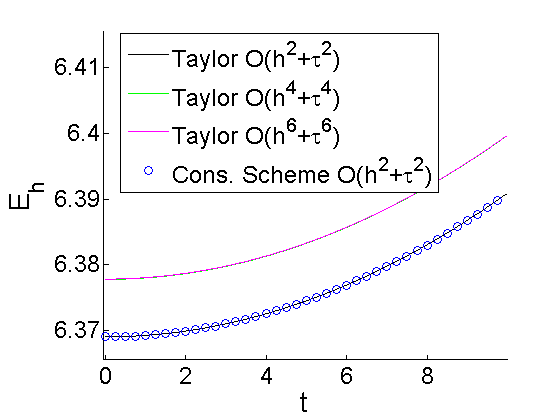
\includegraphics[width=\linewidth]{Mass_bt3_c045_h005_Taylor_Conservative.png}
	\end{minipage}	
	\begin{minipage}[b]{0.4\linewidth}
		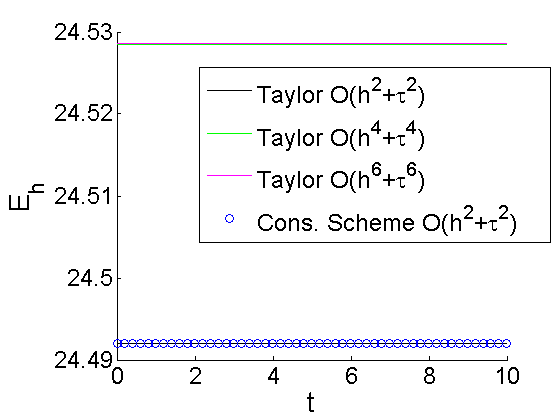
\includegraphics[width=\linewidth]{Energy_bt3_c045_h005_Taylor_Conservative.png}	
	\end{minipage}
\caption{The Mass (left) and Energy (right) of the solution for Test 1, $O(|h|^2 + \tau^2)$ and $T=10$.}
\label{Test1En}
\end{figure}

The Mass increases slightly over the time interval but the gain is neglectable compared to the initial value. For Test 1 the increase with respect to the initial Mass is $0.33\%$ and for Test 2 is $1.8\%$.

\begin{figure}[ht]\vspace{0.2cm}
	\begin{minipage}[b]{0.4\linewidth}
		 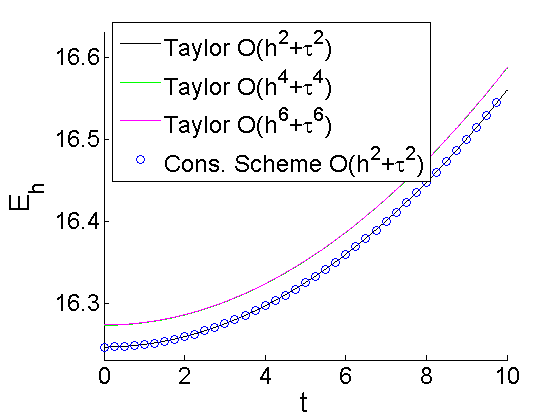
\includegraphics[width=\linewidth]{Mass_bt1_c090_h010_Taylor_Conservative.png}
	\end{minipage}	
	\begin{minipage}[b]{0.4\linewidth}
		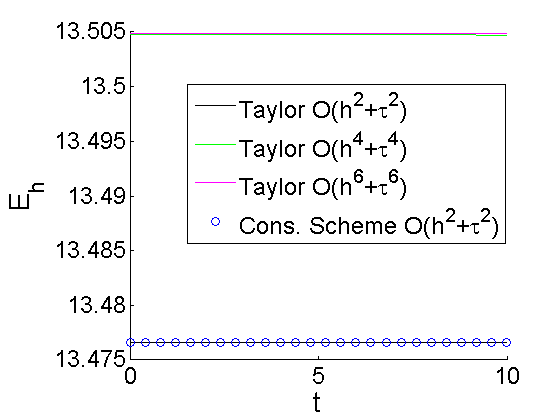
\includegraphics[width=\linewidth]{Energy_bt1_c090_h010_Taylor_Conservative.png}
		
	\end{minipage}
\caption{The Mass (left) and Energy (right) of the solution for Test 2, $O(|h|^2 + \tau^2)$ and $T=10$.}
\label{Test2En}
\end{figure}

For the Taylor Method, the discrete Mass and Energy in Figure \ref{Test1En} and \ref{Test2En} are calculated with three different approximations, namely, trapezoidal formula \rf{quadr2} with $O(h^2)$, Simpson's Rule \rf{quadr4} with $O(h^4)$ and Boole's Rule \rf{quadr6-2D} with $O(h^6)$. It is observed that increasing the order of approximation does not affect the gain for the Mass. It is also confirmed that decreasing the step size $h$ produces similar result, i.e. the graph is slightly shifted upwards or downwards. In the next computations, in order to validate the proper behaviour of the Mass, only the size of the domain is changed whereas the approximation order and discrete steps are fixed.
%----------------------------------------------------------------------------------------------------------------------------------------------
\iffalse
\begin{figure}[ht]\vspace{0.4cm}
	\begin{minipage}[b]{0.33\linewidth}
		 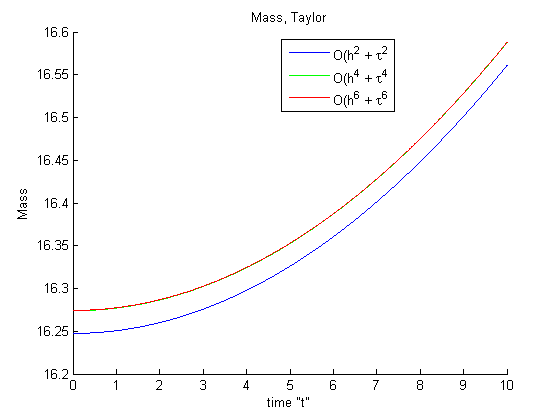
\includegraphics[width=\linewidth]{figures/Mass_bt1_c090_h010_x3O.png}
	\end{minipage}	
	\begin{minipage}[b]{0.33\linewidth}
		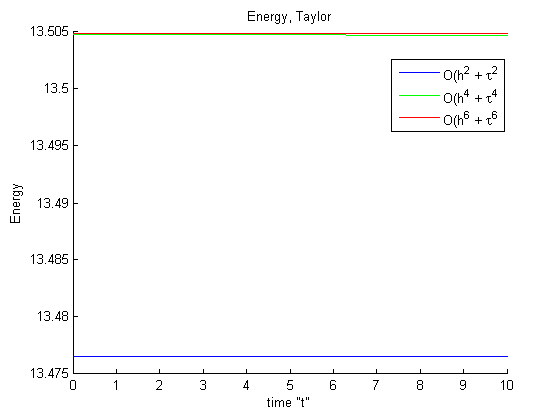
\includegraphics[width=\linewidth]{figures/Energy_bt1_c090_h010_x3O.png}
		
	\end{minipage}
\caption{The Mass (left) and Energy (right) of the Taylor solution for Test 1, $O(|h|^2 + \tau^2)$, $O(|h|^4 + \tau^4)$, $O(|h|^6 + \tau^6)$ and $T=10$.}
\label{Test1TEn}
\end{figure}
\begin{figure}[ht]\vspace{0.4cm}
	\begin{minipage}[b]{0.33\linewidth}
		 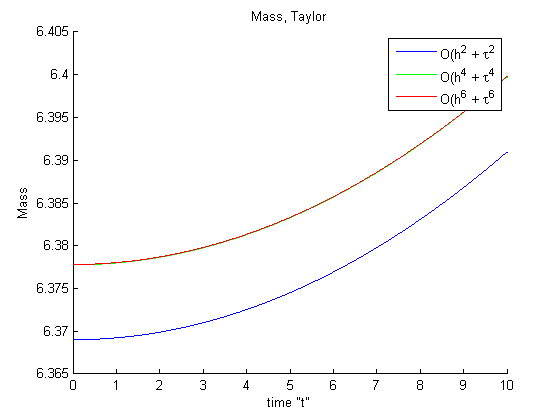
\includegraphics[width=\linewidth]{figures/Mass_bt3_c045_h005_x3O.png}
	\end{minipage}	
	\begin{minipage}[b]{0.33\linewidth}
		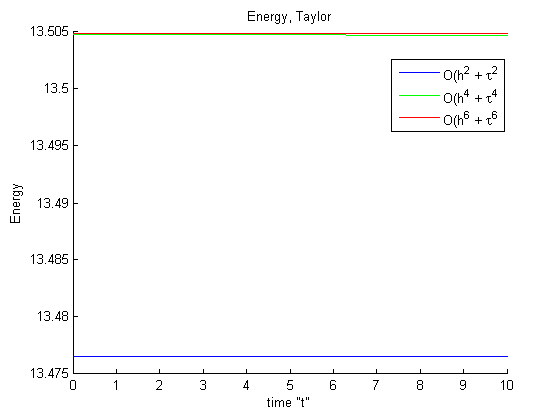
\includegraphics[width=\linewidth]{figures/Energy_bt1_c090_h010_x3O.png}
		
	\end{minipage}
\caption{The Mass (left) and Energy (right) of the Taylor solution for Test 2, $O(|h|^2 + \tau^2)$, $O(|h|^4 + \tau^4)$, $O(|h|^6 + \tau^6)$ and $T=10$.}
\label{Test2TEn}
\end{figure}
\fi
%----------------------------------------------------------------------------------------------------------------------------------------------


\subsection{Numerical Results for the shape of the solution}

The following paragraph discusses the shape of the solution obtained by the Conservative FDS and Taylor method. Both methods are benchmarked on six different grids with space and time steps defined in Table \rf{gridsT}.
\begin{table}[ht]
\centering
\small
		\begin{tabular}{|c|l|l|l|l|l|}
			\hline
                               &           Variant a  &           Variant b     &     \\
			\hline
            Grid 1          &            $h=0.4$  &            $h=0.2$     &    $\tau = 2.5e-04$  \\
			\hline
            %Grid 1a          &            $h=0.4$     &    $\tau = 2.5e-04$  \\
%			\hline
          %  Grid 1b          &            $h=0.2$     &    $\tau = 2.5e-04$  \\
   %			\hline 
           Grid 2         &            $h=0.4$  &   $h=0.2$  &    $\tau =1.0e-06$   \\   
   			\hline 
      %     Grid 2b         &            $h=0.2$  &    $\tau =1.0e-06$   \\    
%	   \hline
   %        Grid 3a          &            $h=0.8$  &    $\tau =6.25e-05$   \\    
%	   \hline
           Grid 3         &            $h=0.8$  &            $h=0.4$  &    $\tau =6.25e-05$   \\    
	   \hline
		\end{tabular}
	\caption{ Space and time steps used to benchmark the Conservative FDS and the Taylor method.}
	\label{gridsT}
\end{table}
The Conservative scheme produces six numerical solutions with second approximation order over the grids in Table \rf{gridsT}, and the Taylor method uses second approximation order on Grid 1 and fourth on Grid 2 and Grid 3. For the last, we used the numerical solutions obtained from the measurement of the convergence speed in Table \rf{tableA}. The end time is $T=10$ and the boundaries of the space domain are $L_1 = L_2 = 60$.

\begin{table}[ht]
\centering
\small
		\begin{tabular}{|c|l|l|l|l|l|l|l|}
			\hline
           Grid                    & Variant   &    $|u_{ex}-u_{T}|_{L2}$  &    $|u_{ex}-u_{C}|_{L2}$  &   $|u_{ex}-u_T|_{\infty}$ &   $|u_{ex}-u_C|_{\infty}$   &  $|u_{ex}|_{\infty}$      \\
			\hline
           Grid 1          &     a:  $h=0.4$  &  $ 7.669196e-04$       &     $7.904798e-04$               &     $5.838980e-04$           &               $6.023530e-04$     &       $1.279362e-01$ \\
			\hline
           Grid 1          &     b:  $h=0.2$  &  $ 1.200402e-04$       &     $1.353479e-04$               &     $1.274495e-04$           &               $1.451817e-04$     &       $1.281769e-01$ \\
			\hline
           Grid 2          &     b:  $h=0.4$  &  $ 9.118794e-06$       &     $1.636122e-03$               &     $7.064211e-06$           &               $1.067977e-03$     &       $1.279362e-01$ \\
			\hline
           Grid 2          &     b:  $h=0.2$  &  $ 3.715136e-07$       &     $ 1.506615e-04$               &     $3.563062e-07$           &               $1.587225e-04$     &       $1.281769e-01$ \\
			\hline
           Grid 3          &     b:  $h=0.8$  &  $ 1.962184e-04$       &     $ 4.630863e-03$               &     $1.058293e-04$           &               $2.537092e-03$     &       $1.278007e-01$ \\
			\hline
           Grid 3          &     b:  $h=0.4$  &  $ 1.044382e-05$       &     $  7.955113e-04$               &     $ 6.808462e-06$           &               $6.066573e-04$     &       $1.279362e-01$ \\
			\hline
		\end{tabular}
	\caption{ Comparison of the Taylor method  $u_{T}$ and the Conservative FDS $u_{C}$ with the exact solution $u_{ex}$.}
	\label{compareTable}
\end{table}

Table \rf{compareTable} compares the numerical solutions from the Taylor method and the Conservative FDS with the exact formula \rf{orgBsqSol}. The first two columns define the type of used grid. The next two columns show the errors of both methods in $L_2$ norms and the next two - errors in $L_\infty$ norms. The last column displays the maximum of the soluiton on the used grid. Decreasing the time or space steps leads to smaller errors
for both methods. For the Grid 1 we used only second approximation order $p=2$ and thus the errors for both methods are similar. Nevertheless for Grid 2 and Grid 3 the Taylor method uses fourth approximation order whereas 
the Conservative FDS uses only second. Thus, the errors measured with the Taylor method are at least $151$ times (or much) smaller on Grid 2 and at least $23$ times (or much) smaller on Grid 3 when compared to the errors from the Conservative FDS. In conclusion, the Taylor method produces finer results with smaller error when $p=4$. Nevertheless, the Conservative FDS is between 100 and 1000 times faster when using bigger time steps $\tau = h / 10$ which is not possibible in the case of the Taylor method because of stability restrictions (see Table \rf{tableConvSeq}).

\iffalse

\begin{figure}[H]\vspace{0.2cm}
	\centering
	\begin{minipage}[b]{0.40\linewidth}
		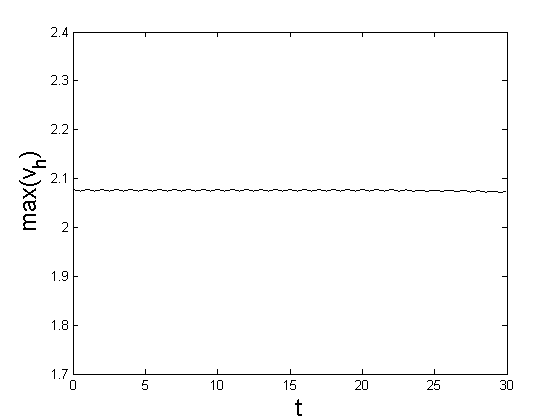
\includegraphics[width=\linewidth]{maximum_30_T30_bt3_c045_h005.png}
	\end{minipage}	
	\begin{minipage}[b]{0.40\linewidth}
		 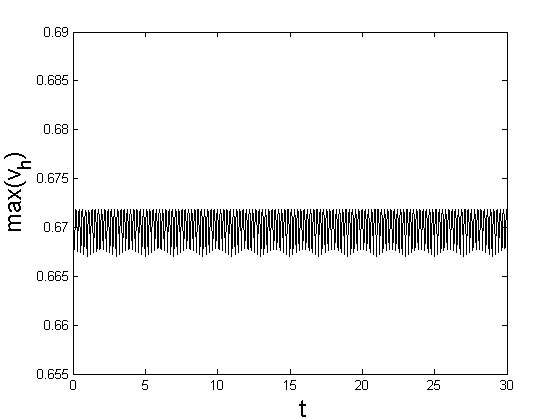
\includegraphics[width=\linewidth]{maximum_30_T30_bt1_c090_h020.png}
	\end{minipage}
\caption{Evolution of the maximum over a larger time interval $[0, 30]$ for Test 1 (left panel) and Test 2 (right panel).}
\label{Maximum}
\end{figure}

\fi

\section{Conclusion}
The 2D BPE is solved using Taylor method with high approximation orders $O(|h|^p + \tau^p)$, $p=2, 4, 6$. The results are compared with the Conservative FDS for $O(|h|^2 + \tau^2)$. Solutions from both methods are qualitatively and quantitatively very similar. Runge's Rule show that the discrete solution and Energy converge for all numerical calculations described in Table \ref{tableP}. The Mass and Energy of the Taylor method are saved with high accuracy over the time interval $[0, 10]$. The discrete Energy is a constant function of the time variable. It is hard to measure the Mass which is defined as an infinite integral of the solution. Computational tests show that the discrete Mass slightly increases as the wave moves. Nevertheless, it is obtained that the gain for the discrete Mass diminishes when the domain $\Omega_h$ grows. The numerical solutions for wave speeds near the upper limit $c_{max} = min(1, \sqrt{\beta_2/\beta_1})$ are stable in form over the time interval $[0, 10]$. It is seen that the change in the shape decreases when the step sizes $h$ and $\tau$ contract or the approximation order $p$ increases. The behaviour of the maximum over a long period of time $[0, 30]$ is preserved with small errors.

%\begin{acknowledgments}
%The work of the second author has been partially supported by the Bulgarian Science Fund under grant K$\Pi$-06-H22/2.
%\end{acknowledgments}

%\nocite{*}
%\bibliography{aipsamp}% Produces the bibliography via BibTeX.

\begin{thebibliography}{99} \normalsize

\bibitem{refHyp} Angelow K., Comparison between two numerical methods for solution of 2D Boussinesq paradigm equation, \emph{AIP Conference Proceedings}, \textbf{2522}, (2022), 090001

\bibitem{ref16} Angelow, K., Kolkovksa, N., Numercal Study of Traveling Wave Solutions to 2D Boussinesq Equation, {\it Serdica J. Computing}, \textbf{13} (2019), 1-16.

\bibitem{ref0} Boussinesq, J.V., Theorie des ondes et des remous qui se propagent le long d'un canal rectangulaire horizontal, en communiquant au liquide contenu dans ce canal des vitesses sensiblement pareilles de la surface au fond.  {\it Journal de Mathematiques Pures et Appliquees}, \textbf{17} (1872), 55-108.

\bibitem{ref21} Chertok, A., Christov, C.I., Kurganov, A., Central-Upwind Schemes for the Boussinesq Paradigm Equations,
{\it Computational Science and High Performance Computing IV, Notes Numer. Fluid Mech.}, \textbf{113} (2011), 267-281.

\bibitem{ref13}  Christou M. , Christov C.I.,
Galerkin spectral method for the 2D solitary waves of Boussinesq paradigm equation,
In: {\it Applications of Mathematics in Technical and Natural Sciences, Sozopol (Bulgaria)},
\emph{AIP Conference Proceedings}, \textbf{1186}, Issue 1 (2009), 217-225.

\bibitem{ref14}  Christou M. , Christov C.I.,
Fourier Galerkin method for 2D solitons of Boussinesq equation,
{\it Mathematics and Computers in Simulation} \textbf{74} (2007), 82-92.

\bibitem{ref1} Christov, C.I., An energy-consistent dispersive shallow-water model,  {\it Wave Motion}, \textbf{34} (2001), 161-174.

\bibitem{ref15} Christov, C.I., Choudhury, J., Perturbation solution for the 2D Boussinesq equation, {\it Mech. Res. Commun.}, \textbf{38} (2011), 274-281.

\bibitem{ref4} Christov, I., Christov, C.I., Physical dynamics of quasi-particles in nonlinear wave equations,
{\it Physics Letters A}, \textbf{372}, Issue 4 (2008),  841-848.

\bibitem{ref20} Christov, C.I., Kolkovska, N., Vasileva, D., On the Numerical Simulation of Un-
steady Solutions for the 2D Boussinesq Paragigm Equation,
{\it In: I. Dimov, S. Dimova, N. Kolkovska (Eds.), Numerical Methods and Applications 2010},
\emph{Conference Proceedings}, \textbf{6046} (2010), 386–394.

\bibitem{ref23} Dimova M., Vasileva D., Comparison of Two Numerical Approaches to Boussinesq Paradigm Equation, 
{\it Lect. Notes Comput. Sci.}, \textbf{8236} (2013), 255-262.

\bibitem{forn}
Fornberg, B., Generation of Finite Difference Formulas on Arbitrarily Spaced Grids, 
Math. Comput., 51(1988),  699 -- 706.

\bibitem{ref25} Kolkovska N., Two families of finite difference schemes for multidimensional Boussinesq paradigm equation, In:
{\it Applications of Mathematics in Technical and Natural Sciences,  Sozopol (Bulgaria)},
\emph{AIP Conference Proceedings}, \textbf{1301} (2010), 395.

\bibitem{ref22} Kolkovska, N., Angelow K., A Multicomponent Alternating Direction Method for Numerical Solving of Boussinesq Paradigm Equation,
In: {\it  I. Dimov, I., Farago, I., Vulkov, L. (eds.) NAA 2012},
\emph{Conference Proceedings}, \textbf{8236} (2013), 371–378.

\bibitem{samarski} Samarskii, A., The Theory of Difference Schemes, Marcel Dekker Inc., New York, 2001.

\bibitem{refHyp} Angelow K., Comparison between two numerical methods for solution of 2D Boussinesq paradigm equation, \emph{AIP Conference Proceedings}, \textbf{2522}, (2022), 090001
%
\end{thebibliography}
\end{document}
%
% ****** End of file aipsamp.tex ******